\documentclass[10pt,aspectratio=169,dvipsnames]{beamer}
\usetheme[]{Berlin}

\setbeamertemplate{footline}{
  \usebeamercolor[fg]{framesource}%
  \usebeamerfont{page number in head}%
  \hspace{0.2cm}
  \small \insertframenumber
  \vspace{0.2cm}
  \doclicenseIcon
}

\setbeamercovered{invisible}

\setbeamersize{text margin left=0.8cm, text margin right=0.8cm}

\setbeamertemplate{footline}[
 myframe number]

% PACKAGES
\usepackage[absolute,overlay]{textpos}
\usepackage[utf8]{inputenc}
\usepackage[official]{eurosym}
\usepackage{booktabs,multicol,multirow,tabularx,array}
\usepackage{subcaption}
\usepackage{parskip}
\usepackage{bm}
\usepackage{tikz}
\usepackage{adjustbox}
\usepackage[super]{nth}
\usepackage[version=4]{mhchem}
\usepackage{siunitx}
\usepackage{tikz}
\usetikzlibrary{calc}


\sisetup{
  detect-all = true
}


\usepackage[
    type={CC},
    modifier={by},
    version={4.0},
]{doclicense}

% HYPERREFERENCES
\usepackage{hyperref}
\hypersetup{
	colorlinks=true,
	citecolor=tub-blue,
	linkcolor=tub-blue,
	urlcolor=tub-blue
}

\usepackage[sfdefault]{roboto}
\usepackage[normalem]{ulem}

% \usepackage[backend=biber,style=numeric-comp]{biblatex}
% \addbibresource{references.bib}

\newcolumntype{R}[1]{>{\raggedleft\arraybackslash}p{#1}}


% GRAPHICS
\graphicspath{
    {graphics/},
  }
\DeclareGraphicsExtensions{.pdf,.jpeg,.png,.jpg}

% FORMATTING
\setlength{\parskip}{6pt}
\linespread{1.1}
\newcommand{\seprule}{\par\noindent\textcolor{black!25}{\rule{\textwidth}{0.4pt}}}

% SOURCES
\setbeamercolor{framesource}{fg=gray}
\setbeamerfont{framesource}{size=\tiny}
\newcommand{\source}[1]{\begin{textblock*}{10cm}(3.6cm,8.25cm)
    \begin{beamercolorbox}[ht=0.5cm,right]{framesource}
        \usebeamerfont{framesource}\usebeamercolor[fg]{framesource} Source: {#1}
    \end{beamercolorbox}
\end{textblock*}}

% \refblock{lines}: references in the same spot on each tool slide, growing upwards from the footer
\newcommand{\refblock}[1]{\begin{textblock*}{14.8cm}[0,1](0.8cm,8.38cm)
		\raggedright\fontsize{6.5}{8}\selectfont\setlength{\parskip}{0.15em}
		#1
	\end{textblock*}}
% \refline{label}{url}{text}: one linked line of a \refblock
\newcommand{\refline}[3]{\textbf{#1:} \href{#2}{#3}\par}
% \prpaper{number}{PR title}{merge date}{paper citation}{paper url}: PyPSA-Eur pull request and related paper
\newcommand{\prpaper}[5]{\refblock{%
		\textbf{PyPSA-Eur PR:} \href{https://github.com/PyPSA/pypsa-eur/pull/#1}{\##1 #2} (merged #3)\par
		\refline{Paper}{#5}{#4}}}

% REFERENCES
% \usepackage[style=nature, doi=true, maxcitenames=3]{biblatex}
% \bibliography{bibliography}
% \renewcommand*{\bibfont}{\footnotesize}

% COLOR TEXT
\newcommand{\bl}[1]{\textcolor{tub-blue}{#1}}
\newcommand{\gr}[1]{\textcolor{tub-green}{#1}}
\newcommand{\rd}[1]{\textcolor{tub-red}{#1}}
\newcommand{\yl}[1]{\textcolor{tub-yellow}{#1}}
% \newcommand{\org}[1]{\textcolor{tub-orange}{#1}}
\newcommand{\cb}[1]{\colorbox{gray!20}{#1}}

\usepackage{array}% https://ctan.org/pkg/array
\makeatletter
\g@addto@macro{\endtabular}{\rowfont{}}% Clear row font
\makeatother
\newcommand{\rowfonttype}{}% Current row font
\newcommand{\rowfont}[1]{% Set current row font
   \gdef\rowfonttype{#1}#1%
}
\newcolumntype{L}{>{\rowfonttype}l}

\usepackage[most]{tcolorbox}
\tcbuselibrary{listingsutf8}

% Custom commands
\usepackage{caption}
\renewcommand{\figurename}{} % Removes the "Figure" text
\captionsetup[figure]{labelformat=empty, labelsep=none} % Removes numbering and colon


% FONT
%\usepackage{utopia}

% REFERENCES
%\usepackage[backend=biber,style=authoryear-comp]{biblatex}
%\bibliography{references.bib}

% DECK-SPECIFIC
\usepackage{fontawesome5}
\usepackage{twemojis}
\usepackage{qrcode}
\colorlet{ink}{black}
\colorlet{mute}{black!60}
\colorlet{rule}{black!25}
\colorlet{inv}{tub-blue}
\colorlet{adv}{tub-red}
\colorlet{rec}{tub-green}
\colorlet{panel}{tub-blue!8}

% take-away line under a figure
\newcommand{\takeaway}[1]{%
  \par\smallskip
  \colorbox{panel}{\parbox{\dimexpr\linewidth-2\fboxsep}{\footnotesize\strut#1\strut}}}

% placeholder box: \placeholder{width}{height}{text}
\newcommand{\placeholder}[3]{%
  \tikz{\node[draw=mute,dashed,thick,fill=panel,rounded corners=2pt,minimum width=#1,
    minimum height=#2,text width=\dimexpr#1-0.4cm\relax,align=center,font=\scriptsize\color{mute}]
    {\faImage\ \textbf{Placeholder}\\[0.2em]#3};}}

% paper thumbnails with markers for where the work comes up today
\colorlet{chipI}{tub-red}
\colorlet{chipII}{tub-blue}
\colorlet{chipPanel}{black!80}
\colorlet{chipPoster}{tub-green}
\newcommand{\chip}[2]{{\setlength{\fboxsep}{1pt}\colorbox{#1}{\fontsize{5.5}{5.5}\selectfont\bfseries\color{white}#2}}}
\newcommand{\chipI}{\chip{chipI}{Research I}}
\newcommand{\chipII}{\chip{chipII}{Research II}}
\newcommand{\chipPanel}{\chip{chipPanel}{Panel}}
\newcommand{\chipPoster}{\chip{chipPoster}{Poster}}
% placed inside a tikzpicture:
% \pageat[markers]{x}{y}{width}{file}{venue}: first page of a paper, top-left corner at (x,y)
\newcommand{\pageat}[6][]{%
  \node[anchor=north west, inner sep=0pt, draw=rule, line width=0.4pt] (pg) at (#2,#3)
    {\includegraphics[width=#4,height=5.6cm,keepaspectratio]{graphics/final-workshop/pages/#5.png}};
  \node[anchor=north west, inner sep=0pt, font=\scriptsize, text=mute, text width=4.4cm,
    align=flush left] at ([yshift=-0.1cm]pg.south west) {#6\ \ #1};}
% \missingat[markers]{x}{y}{width}{height}{venue}{title}: stand-in until a first page exists
\newcommand{\missingat}[7][]{%
  \node[anchor=north west, inner sep=5pt, draw=mute, dashed, line width=0.4pt,
    minimum width=#4, minimum height=#5, text width=\dimexpr#4-12pt\relax, align=flush left,
    font=\scriptsize] (pg) at (#2,#3) {\textbf{#7}\\[0.5em]{\color{mute}first page to be added}};
  \node[anchor=north west, inner sep=0pt, font=\scriptsize, text=mute, text width=4.4cm,
    align=flush left] at ([yshift=-0.1cm]pg.south west) {#6\ \ #1};}
% \topicat{slide}{y}{topic}: black on its own slide, grey otherwise
\newcommand{\topicat}[3]{%
  \alt<#1>{\node[anchor=west, inner sep=0pt] at (0,#2)
      {\textcolor{tub-red}{\rule[0.1ex]{0.85ex}{0.85ex}}\hspace{0.6em}\textbf{#3}};}
    {\node[anchor=west, inner sep=0pt] at (0,#2)
      {\textcolor{black!22}{\rule[0.1ex]{0.85ex}{0.85ex}}\hspace{0.6em}\textcolor{black!35}{#3}};}}

% TITLE PAGE
\title{
  \textbf{Planning in a rollercoaster world:\\three years of RESILIENT}
}
\vspace*{-.5cm}

\institute[Technische Universität Berlin] % (optional, but mostly needed)
{
  \normalsize
  \alert{RESILIENT Final Workshop} \\
  \footnotesize
  Iegor Riepin \\
  Department of Digital Transformation in Energy Systems, TU Berlin \\
  \href{mailto:iegor.riepin@tu-berlin.de}{iegor.riepin@tu-berlin.de} \\
  \vspace{0.3cm}

  20 November 2026
}

\date{}

\subject{RESILIENT Final Workshop}

\titlegraphic{%
\vspace{-1cm}

\includegraphics[height=1cm,clip=true]{graphics/logos/cetp_logo.png}
\hspace{0.7cm}
\includegraphics[trim=0 0cm 0 0cm,height=1cm,clip=true]{graphics/logos/tub_logo.pdf}
\hspace{0.7cm}\raisebox{-0.2cm}{
\includegraphics[trim=0.2cm 0.6cm 0.6cm 0.2cm,height=1.45cm,clip=true]{graphics/logos/bmwe_en_logo.png}}
}

\begin{document}

\addtocounter{framenumber}{-1}
{
	\setbeamertemplate{footline}{
		\usebeamercolor[fg]{framesource}%
		\usebeamerfont{page number in head}%
		\begin{center}
			\Large
			\doclicenseIcon
			\vspace{0.4cm}
		\end{center}
	}
	\maketitle
}

% WHY
\section{Why}
\begin{frame}{We planned this project in one gas crisis and present it in another}
	\centering
	\vspace{-0.3em}
	\includegraphics<1>[width=\linewidth]{graphics/final-workshop/timeline-step1.pdf}%
	\includegraphics<2>[width=\linewidth]{graphics/final-workshop/timeline-step2.pdf}
	\source{Dutch TTF front-month gas price, daily close: ICE Endex, via Yahoo Finance.}
\end{frame}

% QUESTIONS
\section{Questions}
\begin{frame}{Research questions addressed in RESILIENT}
	\small
	\vspace{-0.3em}
	\begin{tikzpicture}[x=1cm, y=1cm]
		\useasboundingbox (0,0.35) rectangle (14.3,-5.95);
		\topicat{1}{0}{Gas price shocks}
		\topicat{2}{-0.75}{Industrial decarbonisation}
		\topicat{3}{-1.5}{Weather extremes}
		\topicat{4}{-2.25}{Biomass and e-fuels}
		\topicat{5}{-3.0}{Trade and geopolitics}
		\topicat{6}{-3.75}{Price formation}
		\topicat{7}{-4.5}{Attacks and outages}
		\only<1>{
			\pageat[\chipI\ \chipPanel]{5.2}{0.3}{4.4cm}{gas}{arXiv, 2026}
		}
		\only<2>{
			\pageat{5.2}{0.3}{4.6cm}{pci}{Environmental Research Letters, 2026}
			\pageat[\chipPoster]{10.1}{0.3}{4.1cm}{nrw}{Case study NRW, 2026}
			\pageat[\chipII\ \chipPoster]{10.1}{-2.55}{4.1cm}{cement}{CEMENT, 2026}
		}
		\only<3>{
			\pageat{5.2}{0.3}{4.7cm}{dunkelflaute}{Applied Energy, 2026}
			\pageat[\chipPoster]{10.2}{0.3}{4.1cm}{edf-pisa-poster}{EDF and University of Pisa, 2026}
		}
		\only<4>{
			\pageat[\chipI\ \chipPoster]{5.2}{0.3}{4.05cm}{biomass}{Nature Energy, 2025}
			\pageat[\chipPoster]{9.6}{0.3}{4.4cm}{ebiofuels}{arXiv, 2026}
			\pageat[\chipPoster]{9.6}{-2.95}{4.1cm}{finland}{Energy, 2026}
		}
		\only<5>{
			\pageat{5.2}{0.3}{4.45cm}{riskindex}{Smart Energy, 2025}
			\pageat{9.85}{0.3}{4.45cm}{pypsaearth}{Applied Energy, 2025}
		}
		\only<6>{
			\pageat{5.2}{0.3}{4.25cm}{priceformation}{Energy Economics, 2025}
		}
		\only<7>{
			\pageat{5.2}{0.3}{4.3cm}{ukraine}{Energy Strategy Reviews, 2025}
			\pageat[\chipI]{5.2}{-3.05}{4.3cm}{selfsufficiency}{Working paper, 2026}
			\pageat{9.8}{0.3}{4.4cm}{osmgrid}{Scientific Data, 2025}
		}
	\end{tikzpicture}
\end{frame}

% UKRAINE
\section{Ukraine}
\begin{frame}{In 2022 we extended PyPSA-Eur to Ukraine and Moldova}

	\begin{columns}[T,onlytextwidth]
		\begin{column}{0.32\textwidth}
			\footnotesize
			In 2022, our group extended \alert{PyPSA-Eur} to cover \alert{Ukraine and Moldova} --- to support work on Ukraine's energy crisis caused by the Russian full-scale invasion.

			\vspace{0.4cm}
			Several research groups have built upon this data extension:
			\begin{itemize}
				\item \href{https://greendealukraina.org/}{Green Deal Ukraine}
				\item \href{https://doi.org/10.1016/j.egycc.2024.100170}{Sotnyk et al., 2024}
				\item \href{https://doi.org/10.1016/j.esr.2025.101724}{Zachmann et al., 2025}
				\item \href{https://doi.org/10.1088/2634-4505/ad6738}{Tröndle et al., 2024}
				\item \href{https://epg.eng.ox.ac.uk/media/ps3nfxzp/report-modelling-framework-and-interlinkages.pdf}{Oxford EPG report}
			\end{itemize}
		\end{column}
		\begin{column}{0.66\textwidth}
			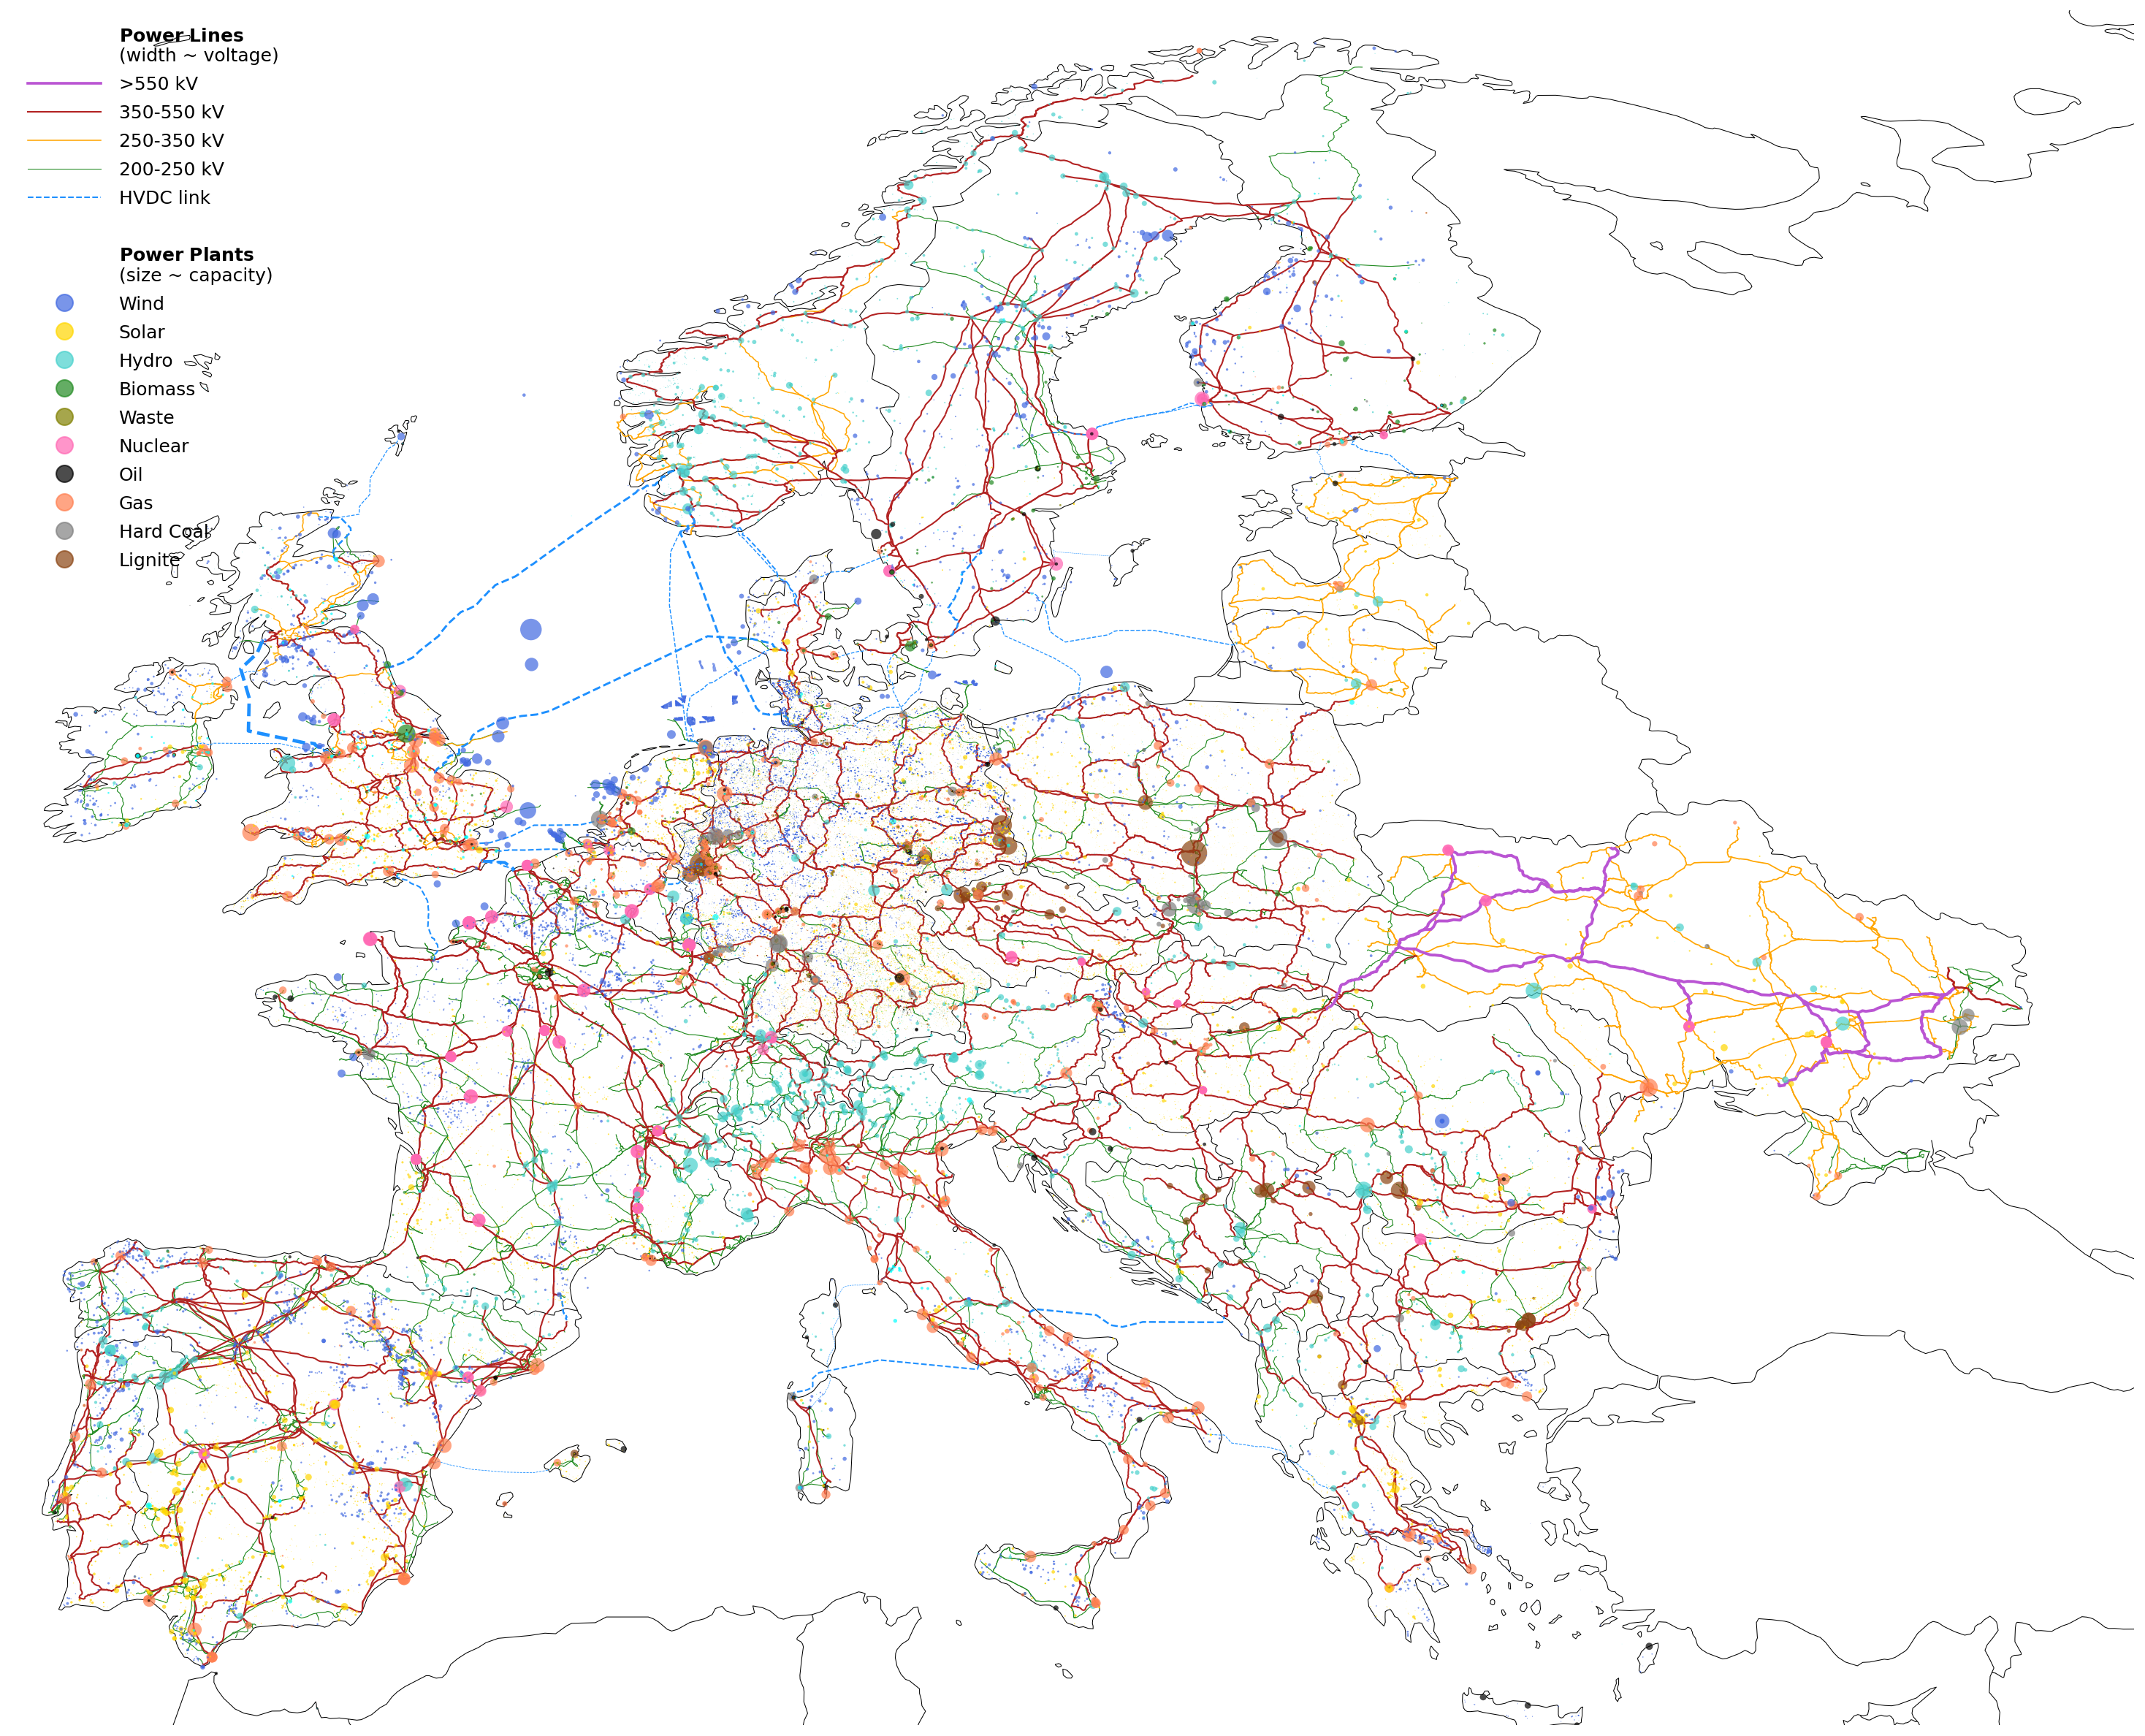
\includegraphics[width=\linewidth]{graphics/pypsa-eur.png}
		\end{column}
	\end{columns}

	\source{\href{https://github.com/PyPSA/pypsa-eur}{PyPSA-Eur} contributors (MIT License)}

\end{frame}

\begin{frame}{Ukraine: what an electricity system under attack needs first}

	\vspace*{-1ex}

	\begin{columns}[T,onlytextwidth]

		\begin{column}{0.55\textwidth}
			\begin{minipage}[t][0.425\textheight][t]{\linewidth}
				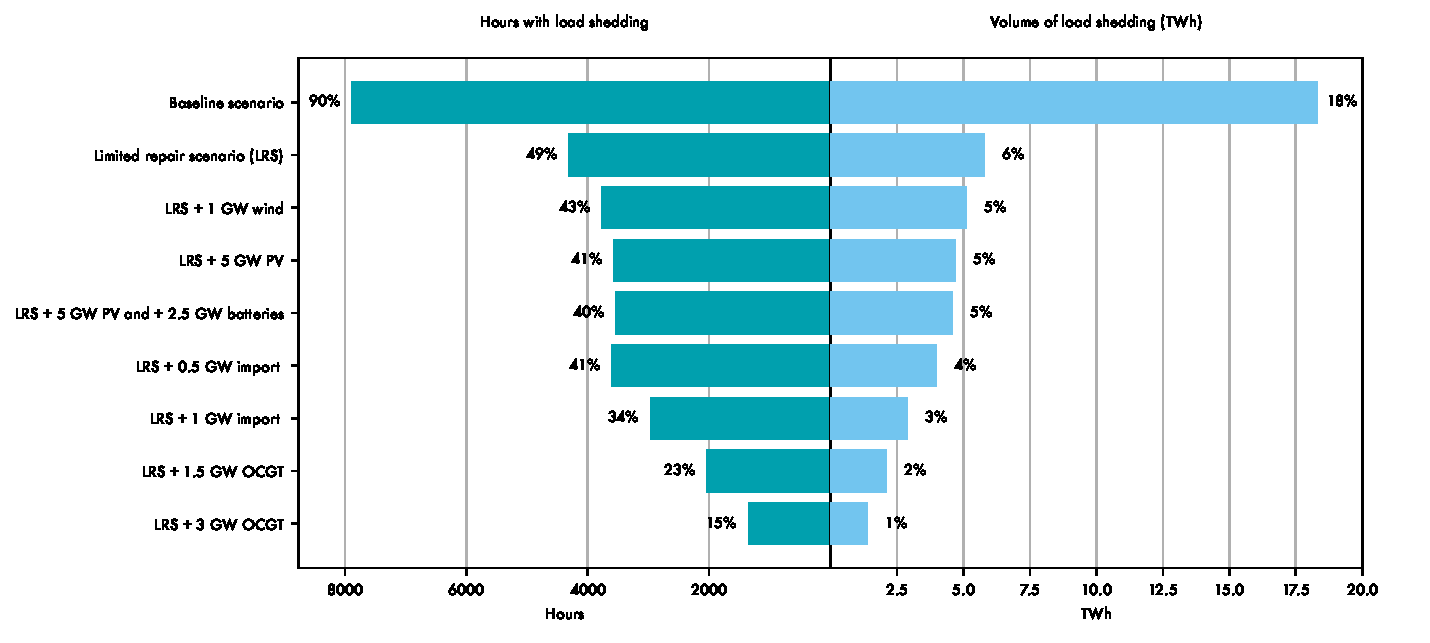
\includegraphics[width=\linewidth,keepaspectratio]{graphics/gdu_comparison.pdf}
			\end{minipage}
			\vfill
			\begin{minipage}[t][0.425\textheight][t]{\linewidth}
				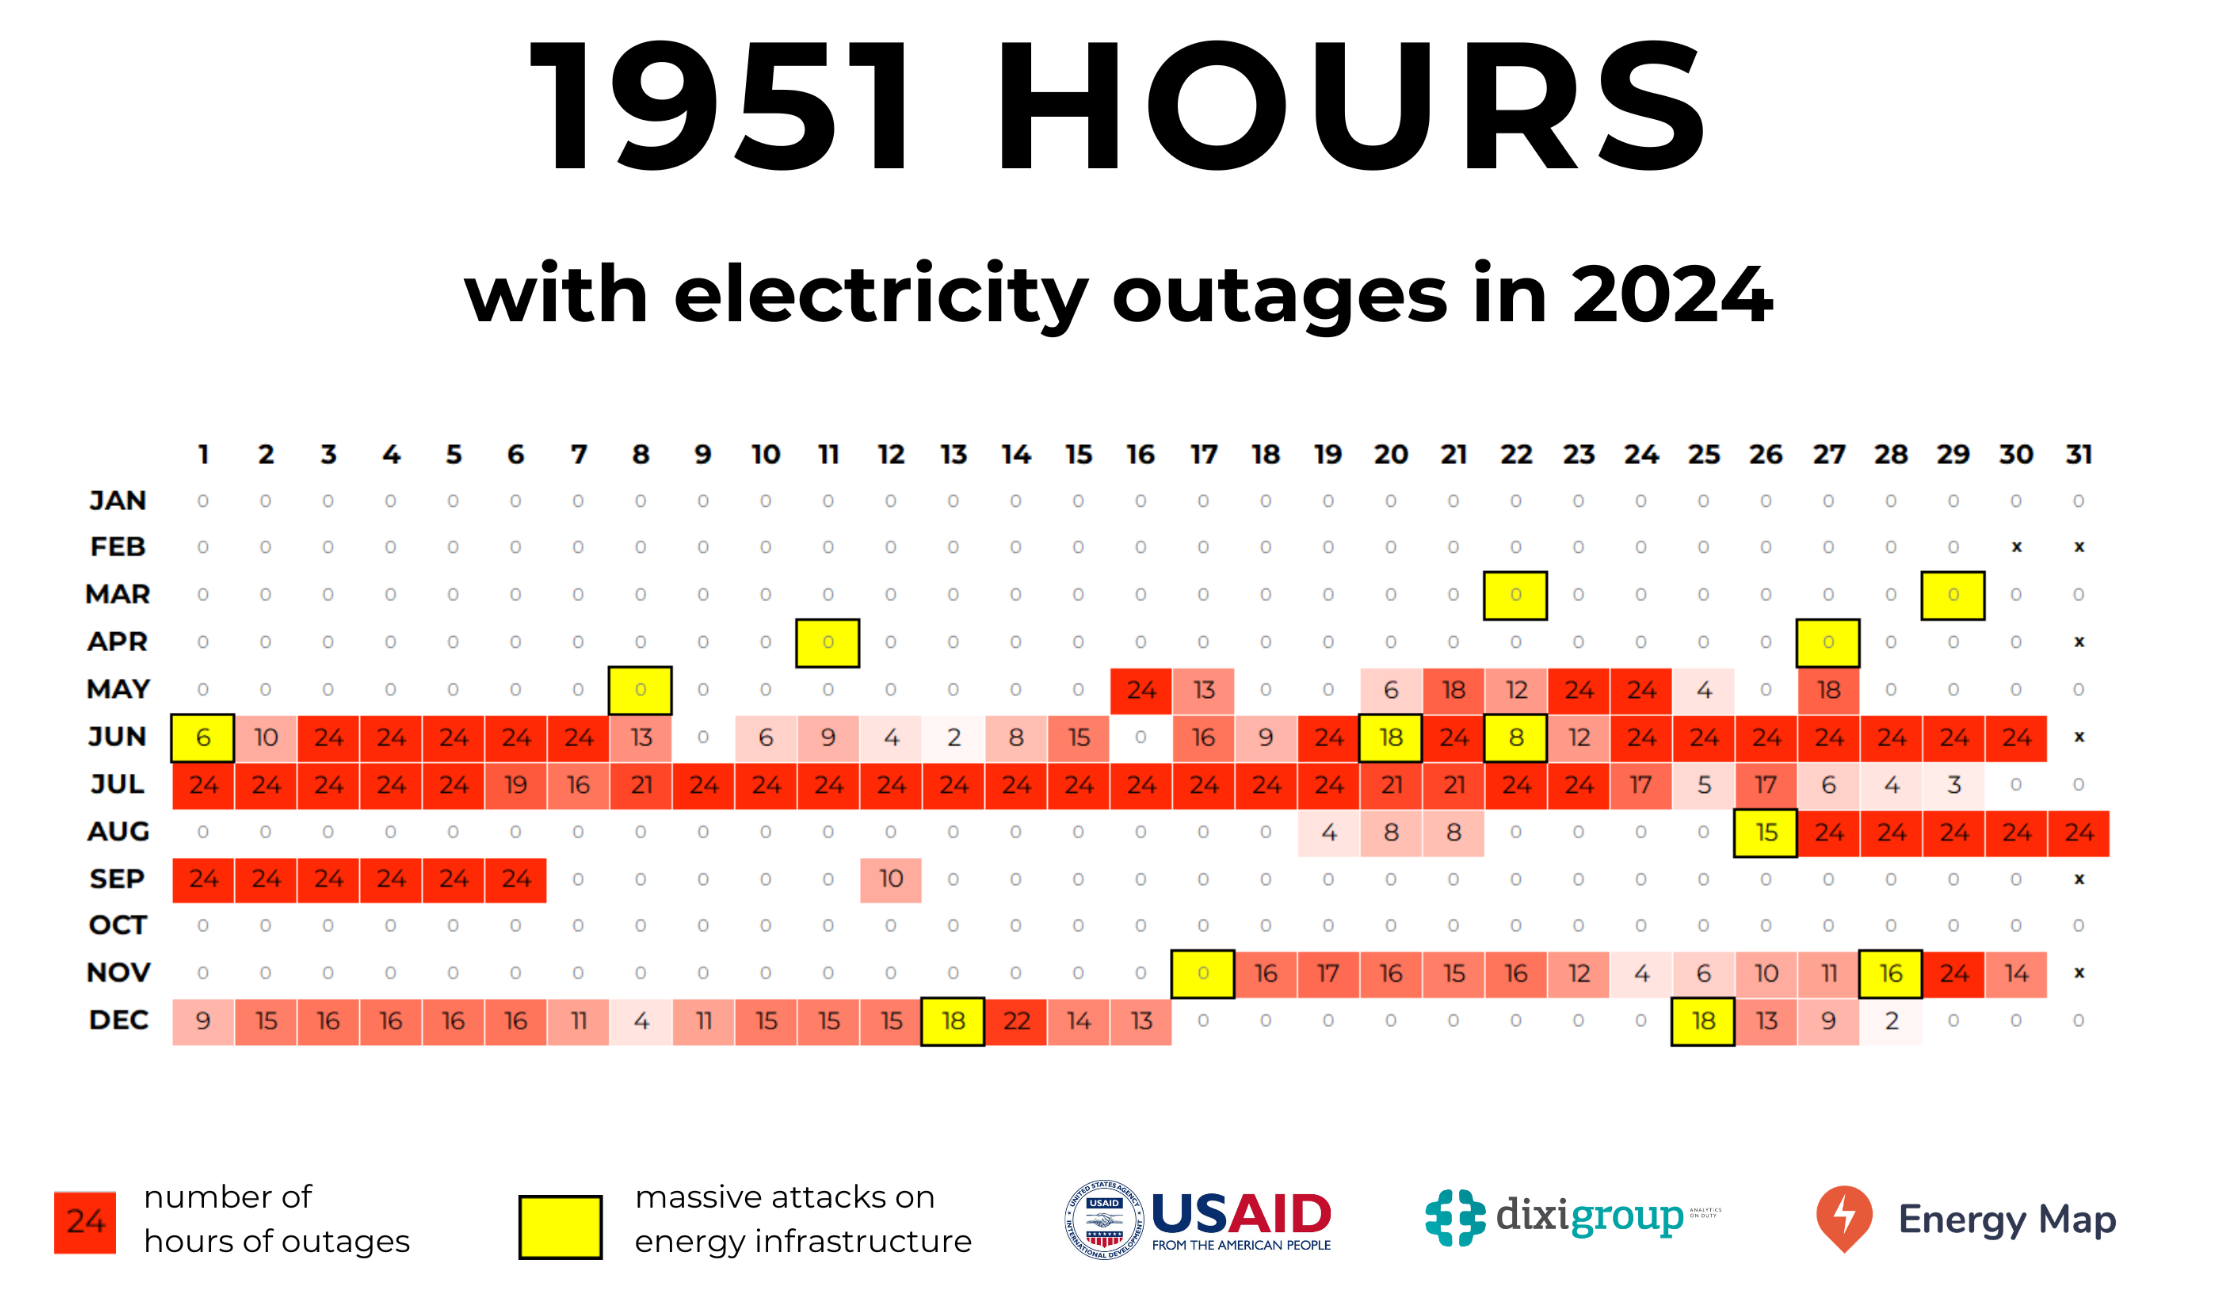
\includegraphics[width=0.9\linewidth,keepaspectratio]{graphics/dixi.png}
			\end{minipage}
		\end{column}

		\begin{column}{0.44\textwidth}
			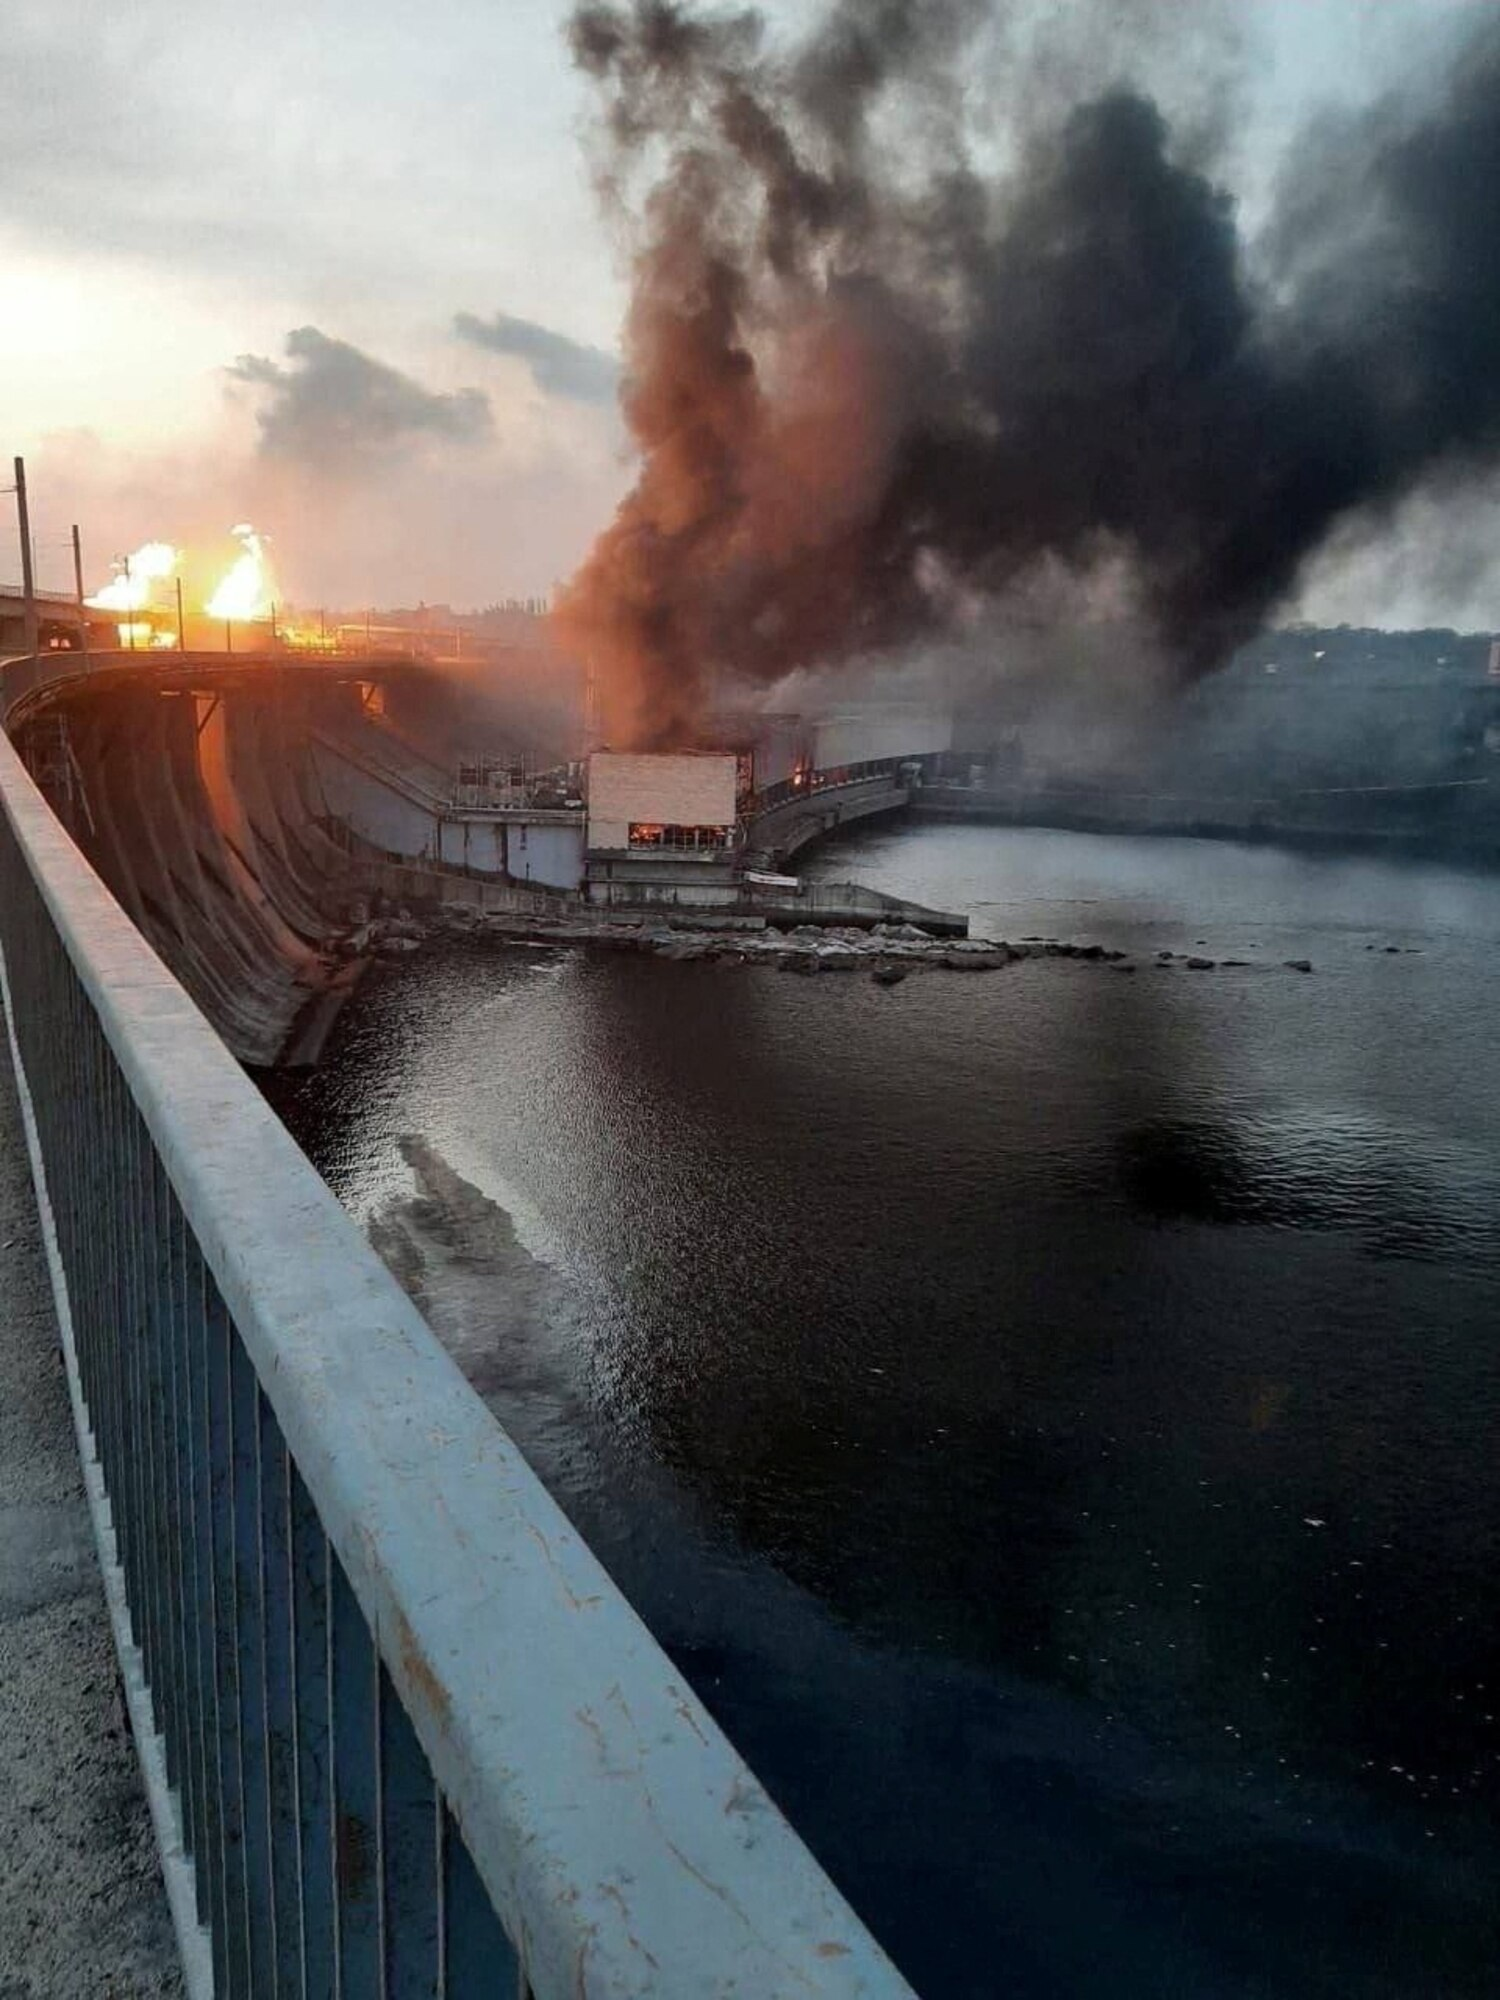
\includegraphics[height=0.85\textheight]{graphics/Dniprohes-strike.png}
		\end{column}
	\end{columns}

	\begin{textblock*}{6.4cm}(8.8cm,8.15cm)
		\raggedleft\usebeamerfont{framesource}\usebeamercolor[fg]{framesource}
		Source: Photo: Reuters (Denys Shmyhal); top: \href{https://doi.org/10.1016/j.esr.2025.101724}{Zachmann, Meißner, Riepin (2025)};\\
		bottom: \href{https://dixigroup.org/en/electricity-outages-lasted-2-thousand-hours-for-ukrainian-households-in-2024/}{dixigroup.org}
	\end{textblock*}

\end{frame}

% TOOLS
\section{Tools}
\begin{frame}{Europe's transmission grid from OpenStreetMap data}
	\centering
	\vspace{-0.6em}
	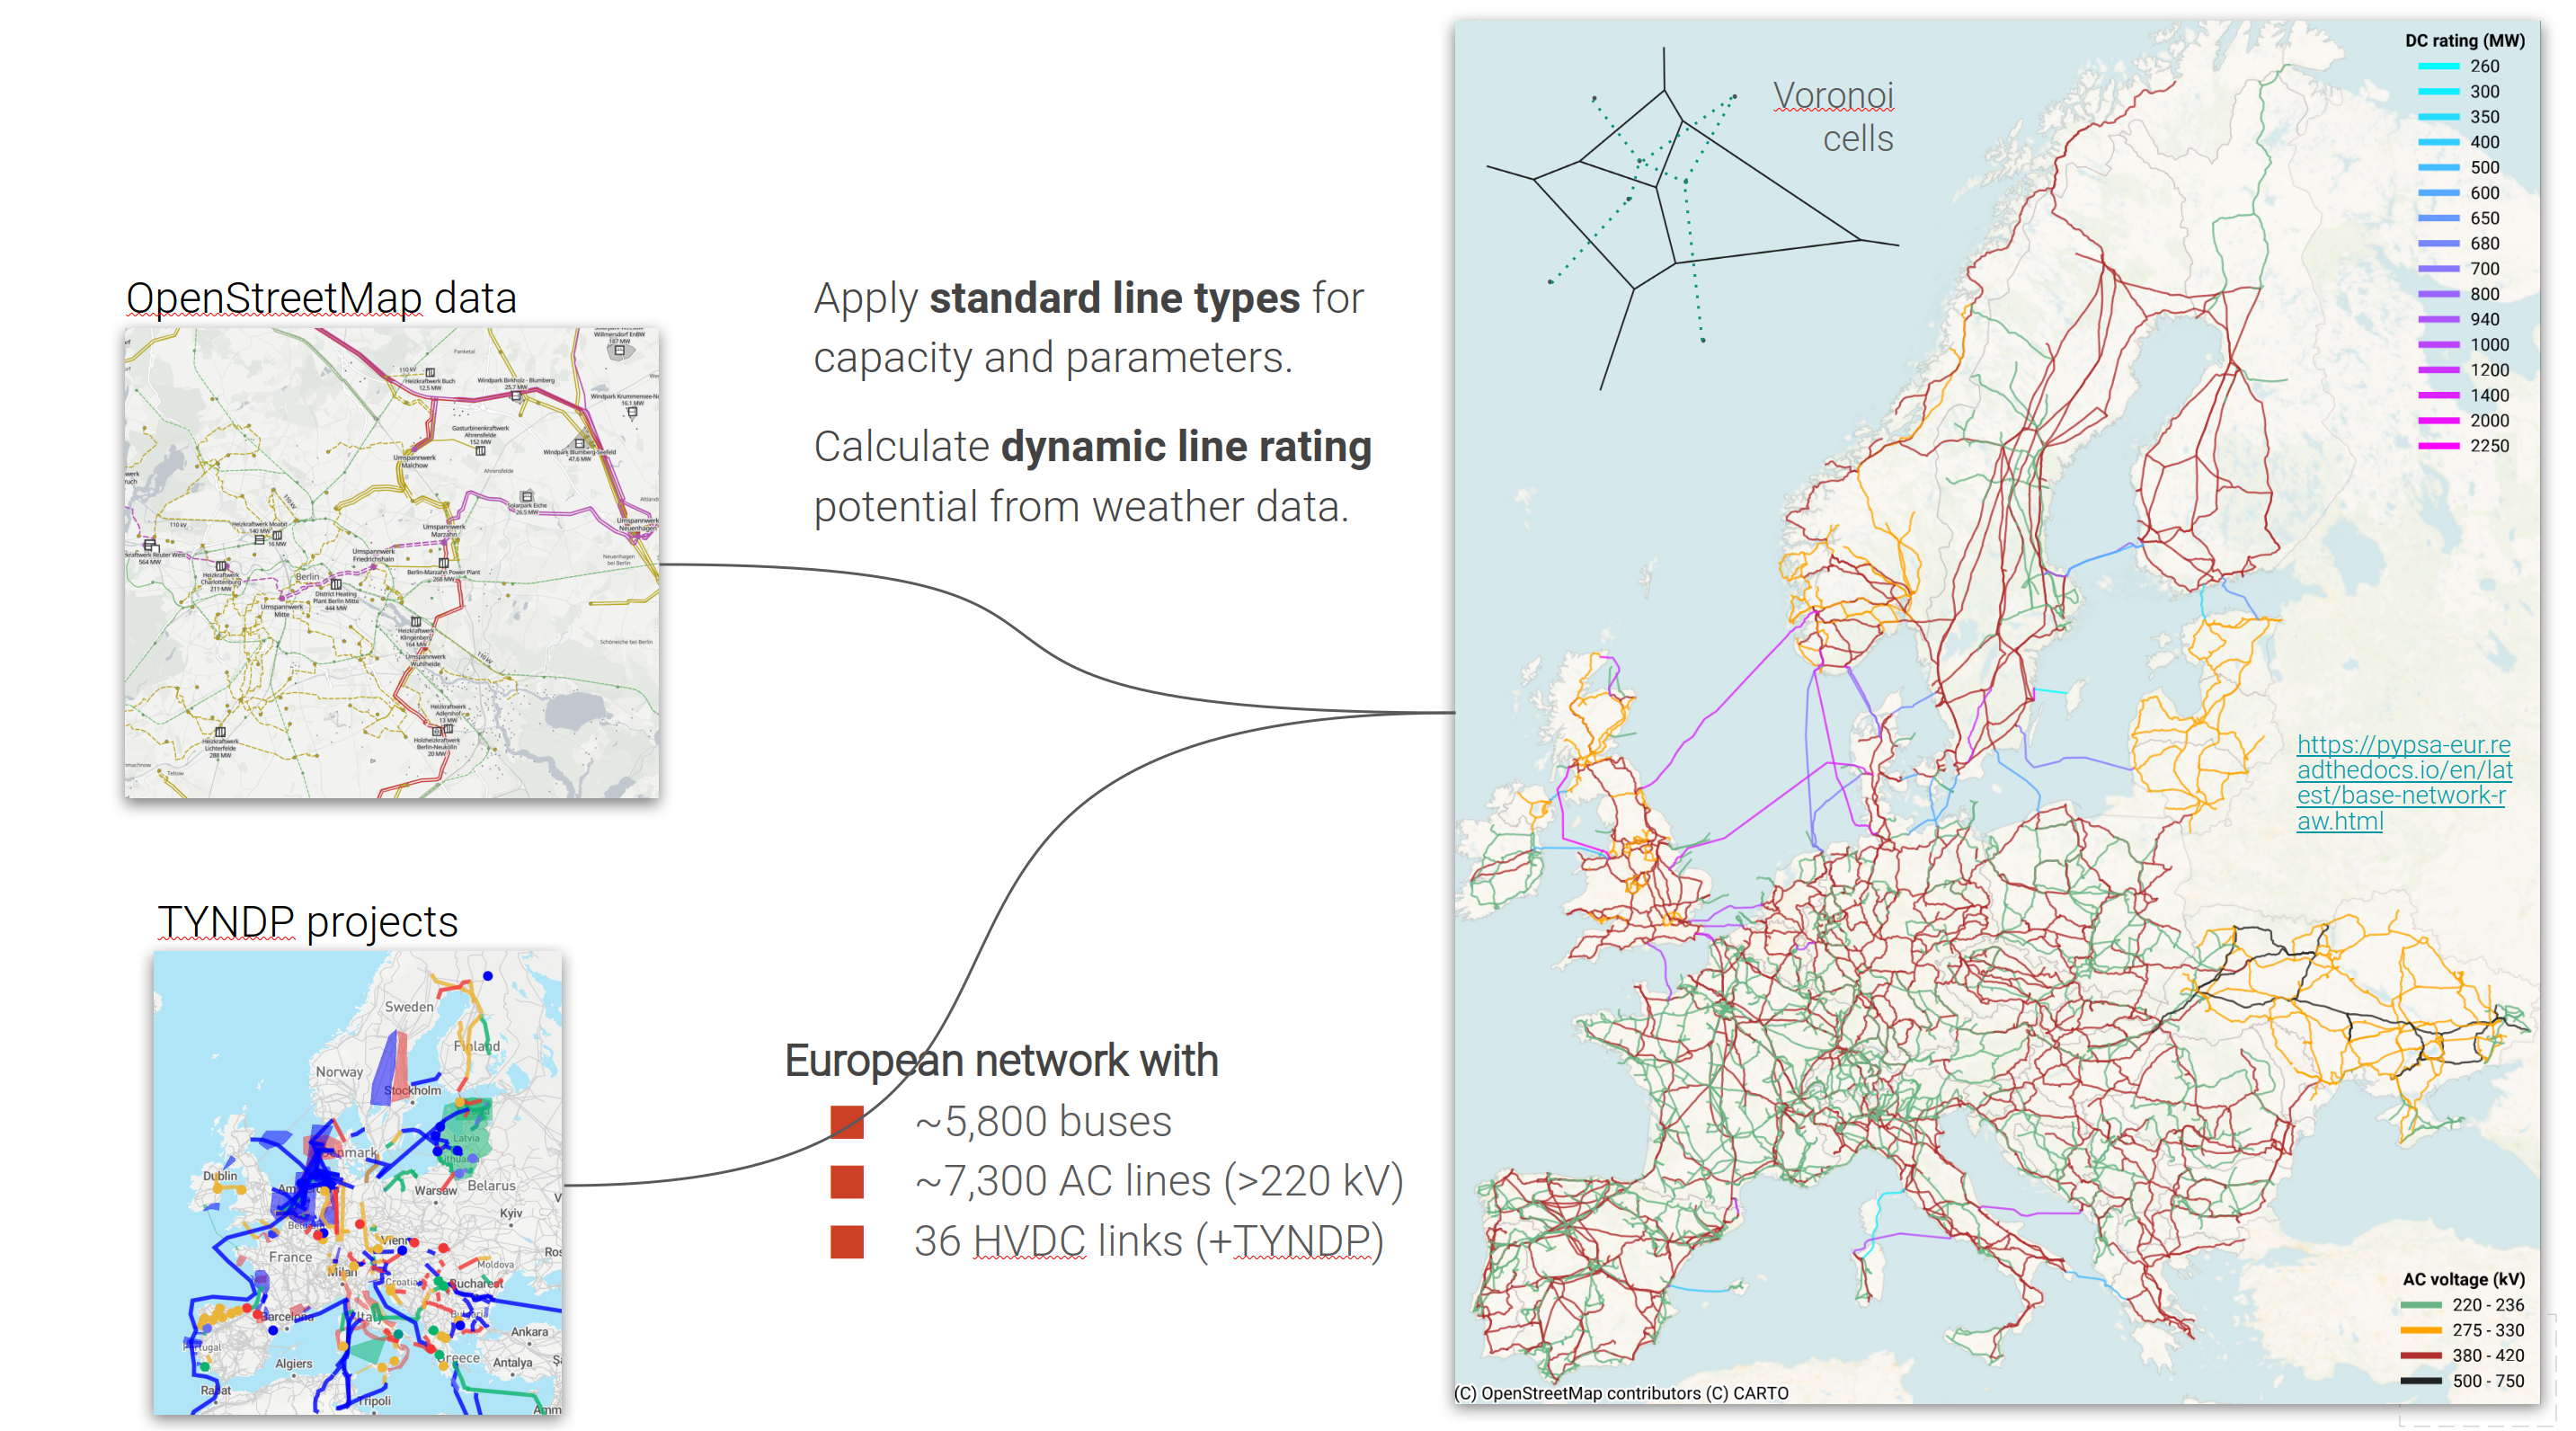
\includegraphics[height=5.55cm]{graphics/final-workshop/osm-grid.png}
	\refblock{%
		\textbf{PyPSA-Eur PR:} \href{https://github.com/PyPSA/pypsa-eur/pull/1079}{\#1079 Introducing OpenStreetMap high-voltage grid to PyPSA-Eur} (merged August 2024)\par
		\textbf{PyPSA-Eur PR:} \href{https://github.com/PyPSA/pypsa-eur/pull/1740}{\#1740 Implementation of voltage levels 110kV-220kV using osm-raw} (merged August 2025)\par
		\refline{Paper}{https://doi.org/10.1038/s41597-025-04550-7}{Xiong et al. (2025). Modelling the high-voltage grid using open data for Europe and beyond. Sci. Data}}
\end{frame}

\begin{frame}{Multiple weather years in one optimisation problem}
	\vspace{-0.5em}
	\begin{columns}[c,onlytextwidth]
		\begin{column}{0.74\textwidth}
			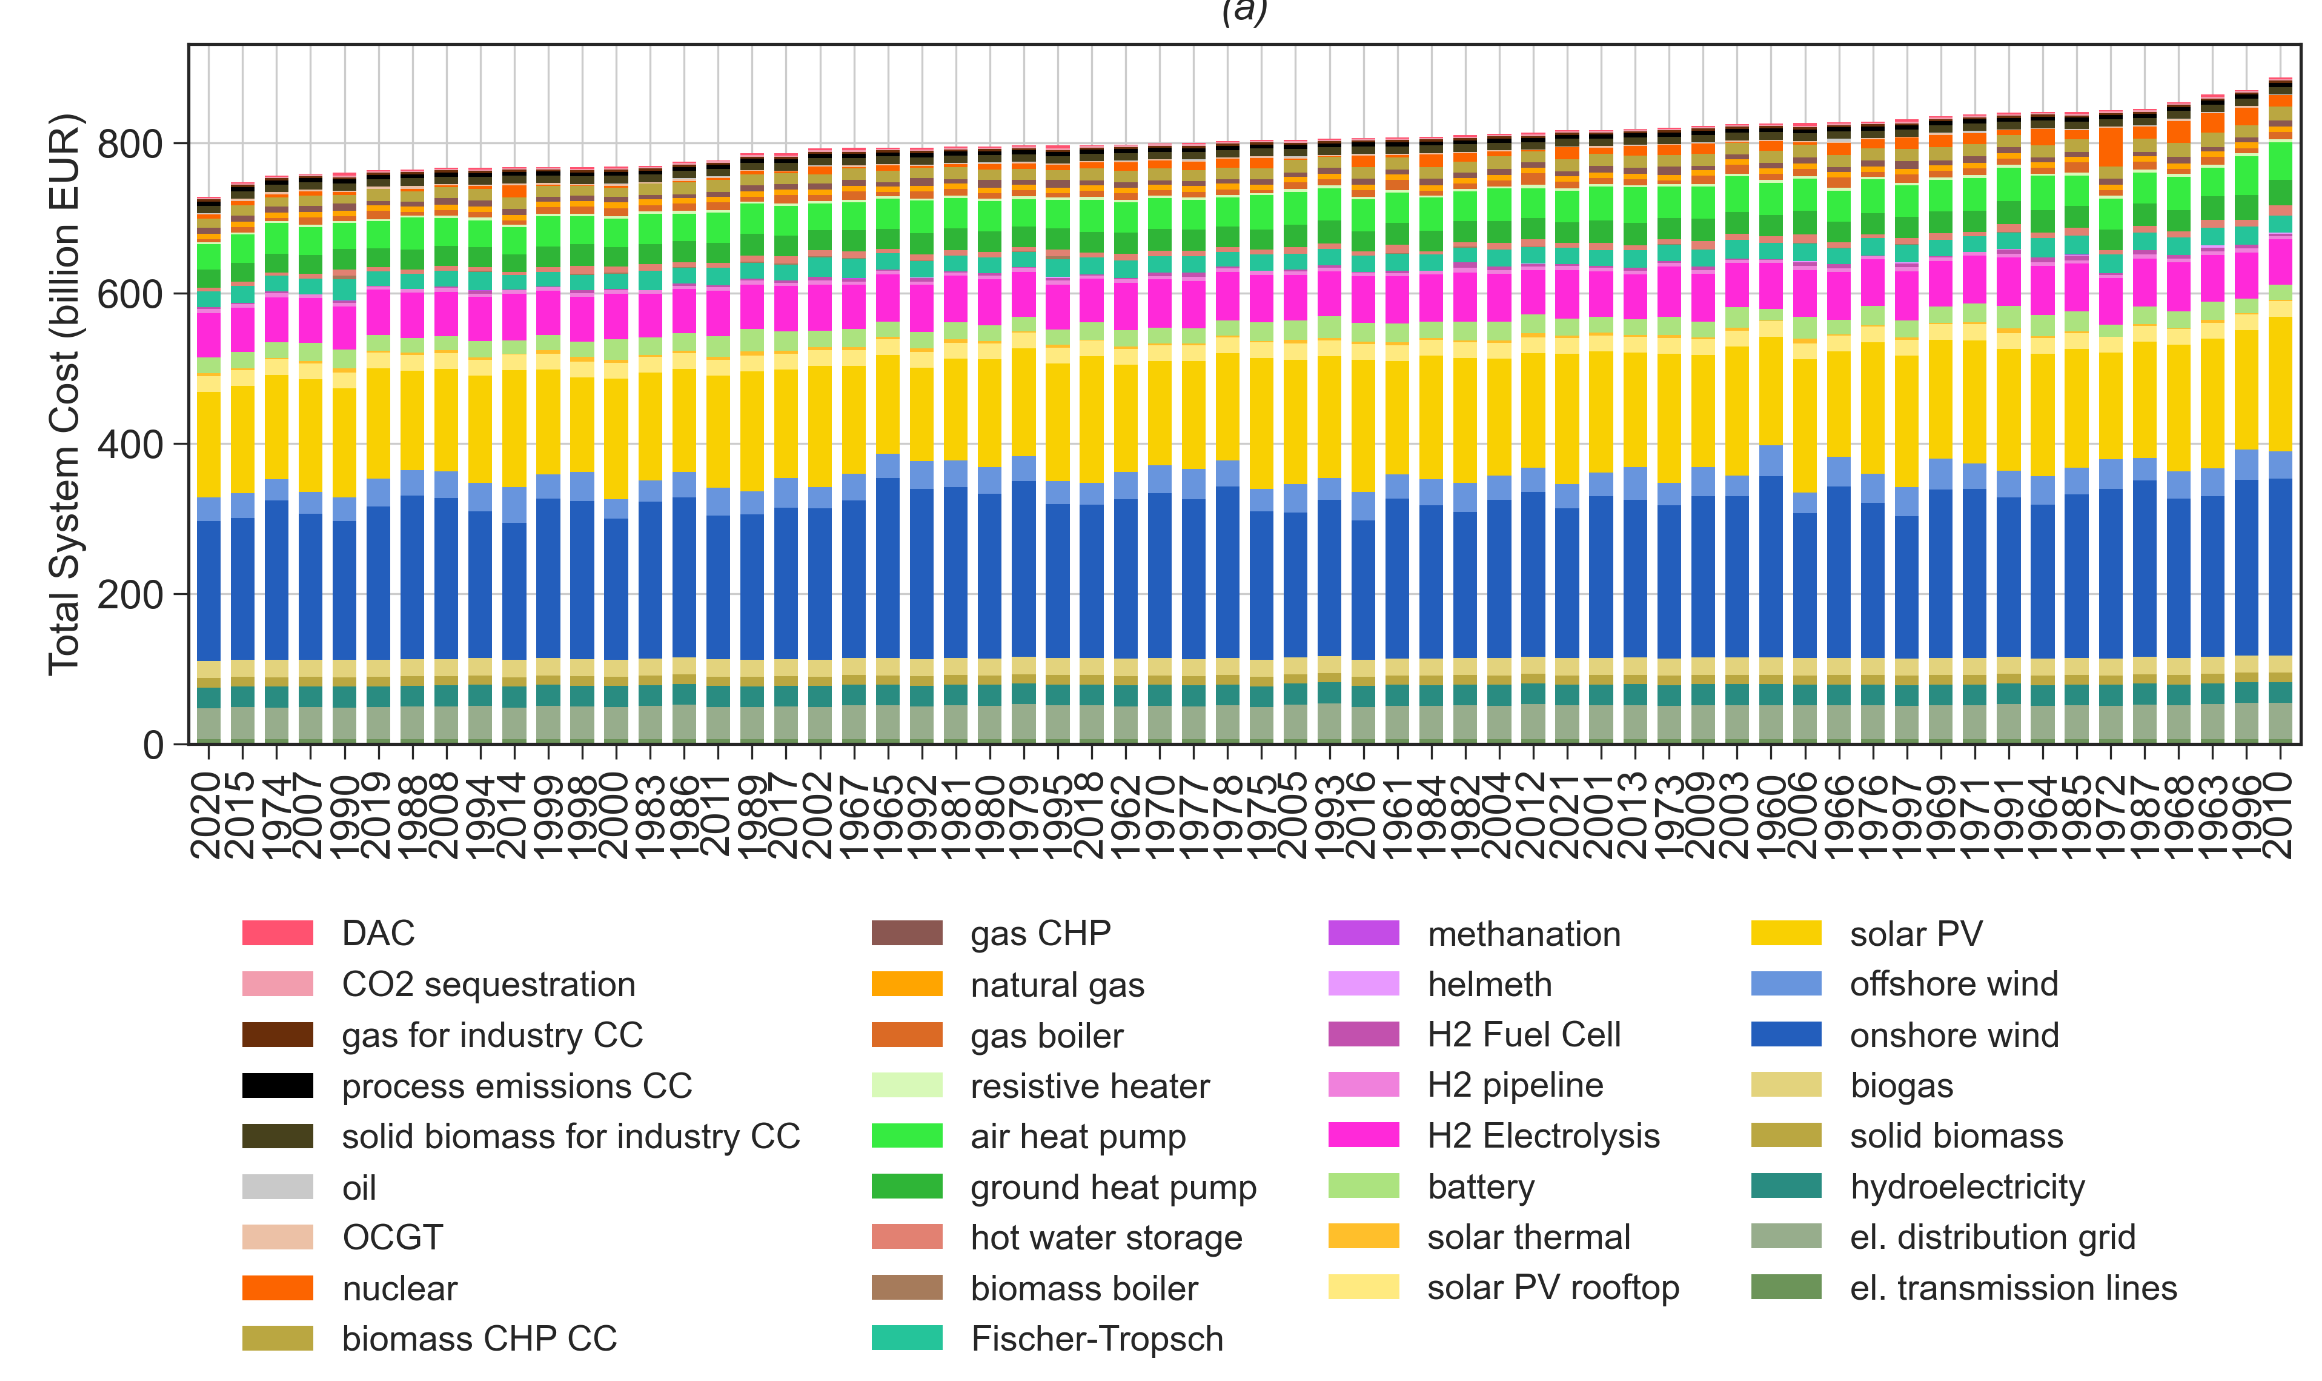
\includegraphics[height=5.9cm]{graphics/tsc-weatheryears.png}
		\end{column}
		\begin{column}{0.24\textwidth}
			\footnotesize
			The cost-optimal system depends on the weather year it is designed for.

			PyPSA-Eur can now optimise one system against \alert{several weather years at once}.
		\end{column}
	\end{columns}
	\prpaper{1613}{Multiple weather years in one optimisation problem}{April 2025}{G{\o}tske et al. (2024). Designing a sector-coupled European energy system robust to 60 years of historical weather data. Nat. Commun.}{https://doi.org/10.1038/s41467-024-54853-3}
\end{frame}

\begin{frame}{Industrial process heat by temperature band}
	\vspace{-1.2em}
	\begin{columns}[c,onlytextwidth]
		\begin{column}{0.34\textwidth}
			\small
			\begin{itemize}\setlength{\itemsep}{0.6em}
				\item Before: industrial heat was a \alert{fixed demand} with fixed fuels
				\item Now: demand is split into \alert{temperature bands}, by industry branch
				\item The model \alert{chooses the supply}: heat pumps, electric boilers, biomass, methane, hydrogen
			\end{itemize}
		\end{column}
		\begin{column}{0.64\textwidth}
			\centering
			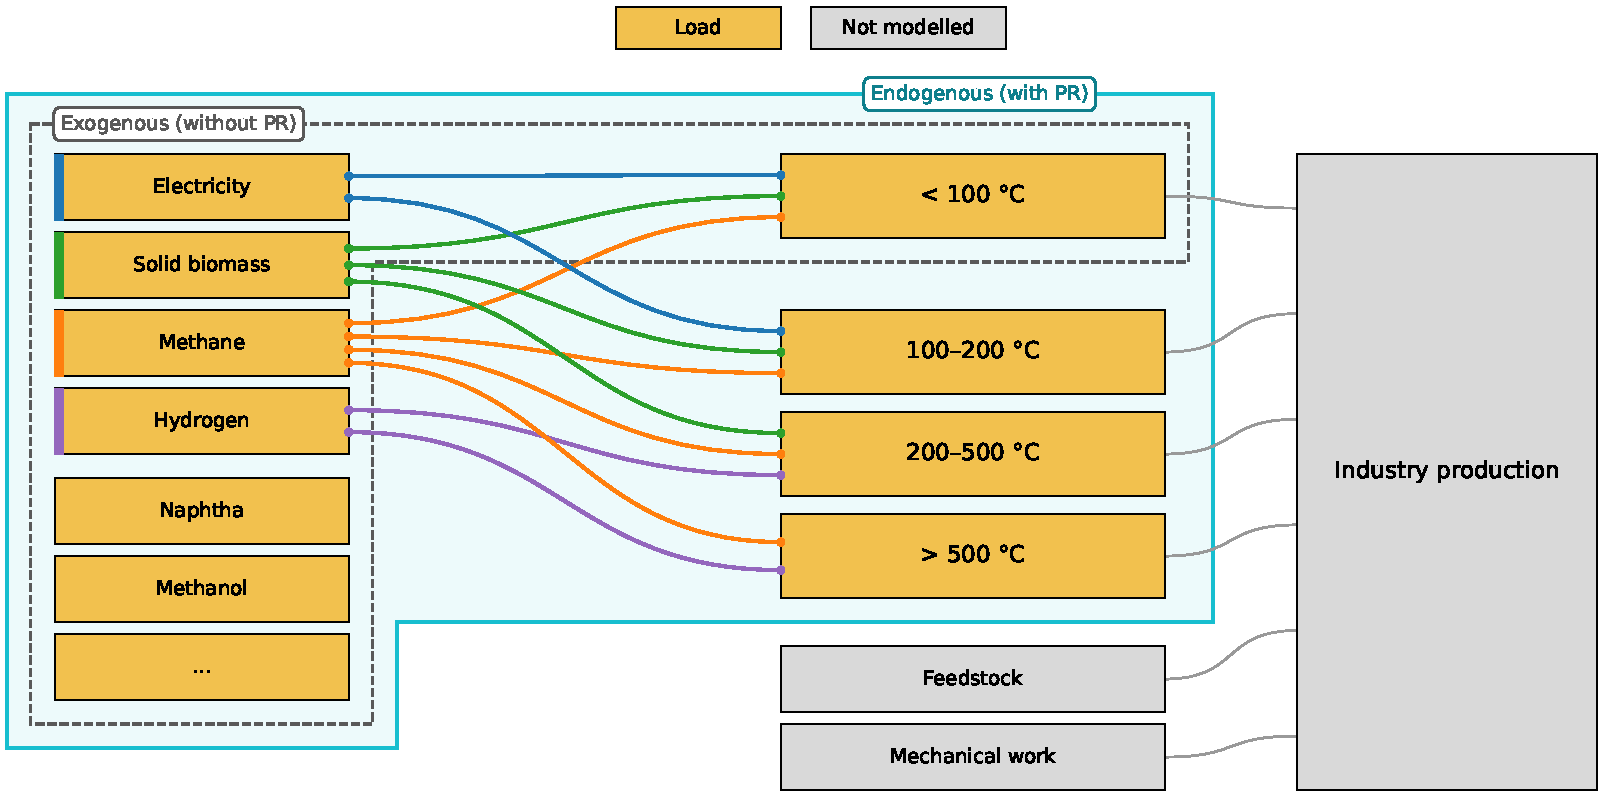
\includegraphics[width=\linewidth]{graphics/final-workshop/industry-heat-supply.pdf}
		\end{column}
	\end{columns}
	\prpaper{1943}{Endogenous Industry Heat}{November 2026}{Franken et al. (2026). Accelerating fossil gas independence in Europe. arXiv}{https://arxiv.org/abs/2607.21048}
\end{frame}

\begin{frame}{Stochastic and risk-averse optimisation, released with PyPSA v1.0}
	\centering
	\vspace{-0.8em}
	\begin{tikzpicture}[x=0.98cm, y=1.0cm, font=\footnotesize,
			dec/.style={circle, draw=black!70, fill=white, line width=0.6pt, inner sep=0pt, minimum size=6pt},
			scen/.style={circle, draw=tub-yellow, fill=tub-yellow!25, line width=0.6pt, inner sep=0pt, minimum size=6pt},
			worst/.style={circle, draw=tub-red, fill=tub-red!30, line width=0.6pt, inner sep=0pt, minimum size=6pt}]
		\node[font=\scriptsize\bfseries, text=mute] at (0.2, 2.45) {investment};
		\node[font=\scriptsize\bfseries, text=mute, align=center] at (2.6, 2.55) {uncertainty\\resolves};
		\node[font=\scriptsize\bfseries, text=mute, align=center] at (5.0, 2.55) {operation in\\each scenario};
		\draw[dotted, draw=mute, line width=0.6pt] (2.6, 2.2) -- (2.6, -2.2);

		% risk-neutral
		\node[anchor=east, align=right] at (-0.25, 1.2) {two-stage,\\\textbf{risk-neutral}};
		\node[dec] (a1) at (0.2, 1.2) {};
		\node[dec] (b1) at (2.6, 1.2) {};
		\draw[line width=0.6pt] (a1) -- (b1);
		\foreach \k in {0,...,5} {
				\node[scen] (s\k) at (5.0, 2.0 - 0.32*\k) {};
				\draw[draw=tub-yellow, line width=0.5pt] (b1) -- (s\k);
			}
		\node[anchor=west] at (5.7, 1.2) {$\min\; \mathrm{CAPEX} + \displaystyle\sum_{s} p_s \cdot \mathrm{OPEX}_s$};

		% risk-averse
		\node[anchor=east, align=right] at (-0.25, -1.2) {two-stage,\\\textbf{risk-averse}};
		\node[dec] (a2) at (0.2, -1.2) {};
		\node[dec] (b2) at (2.6, -1.2) {};
		\draw[line width=0.6pt] (a2) -- (b2);
		\foreach \k in {0,...,3} {
				\node[scen] (t\k) at (5.0, -0.4 - 0.32*\k) {};
				\draw[draw=tub-yellow, line width=0.5pt] (b2) -- (t\k);
			}
		\foreach \k in {4,5} {
				\node[worst] (t\k) at (5.0, -0.4 - 0.32*\k) {};
				\draw[draw=tub-red, line width=0.5pt] (b2) -- (t\k);
			}
		\node[anchor=west] at (5.7, -1.2) {$\min\; \mathrm{CAPEX} + \rd{(1-\omega)}\displaystyle\sum_{s} p_s \cdot \mathrm{OPEX}_s + \rd{\omega \cdot \mathrm{CVaR}_\alpha}$};
	\end{tikzpicture}

	\refblock{%
		\textbf{PyPSA PR:} \href{https://github.com/PyPSA/PyPSA/pull/1154}{\#1154 New Optimization Module \& Stochastic Networks} (merged August 2025)\par
		\textbf{PyPSA PR:} \href{https://github.com/PyPSA/PyPSA/pull/1345}{\#1345 Add risk-averse optimization} (merged September 2025)\par
		\textbf{Case study:} EDF R\&D and University of Pisa. Optimising a large-scale European power network (poster)\par}
\end{frame}

\begin{frame}{Solving it at scale, with the University of Pisa}
	\vspace{-1.6em}
	\begin{columns}[c,onlytextwidth]
		\begin{column}{0.58\textwidth}
			\centering
			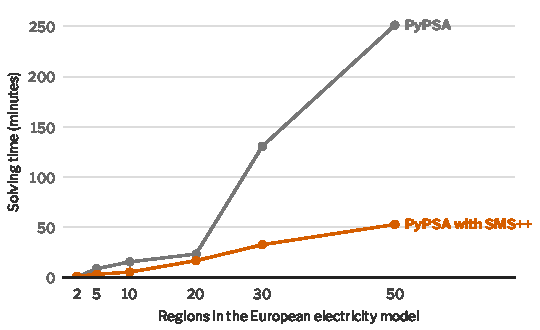
\includegraphics[height=4.7cm]{graphics/final-workshop/smspp-benchmark.pdf}
		\end{column}
		\begin{column}{0.38\textwidth}
			\small
			\begin{itemize}\setlength{\itemsep}{0.6em}
				\item PyPSA now talks to \alert{SMS++}, a framework for \alert{decomposition}
				\item Same optimal solution; solving time grows slower with increasing problem size
				\item Small subproblems make large models tractable also without commercial solvers
			\end{itemize}
		\end{column}
	\end{columns}
	\refblock{%
		\textbf{PyPSA PR:} \href{https://github.com/PyPSA/PyPSA/pull/1558}{\#1558 Smspp optimization} (in review)\par
		\refline{SMS++ development}{https://gitlab.com/smspp/smspp-project}{gitlab.com/smspp/smspp-project}
		\twemoji{1f3c6} \href{https://resilient-project.github.io/static/uploads/062026_hackaton_pipssms.pdf}{Enrico Calandrini (University of Pisa) wins second place at the PEREGRINE PIPS-IPM++ Hackathon for integrating PIPS-IPM++ into SMS++}\par}
\end{frame}

% PEOPLE
\section{People}
% Participant groups, coloured as on the participant map (Okabe-Ito)
\definecolor{grp-research}{HTML}{0072B2}
\definecolor{grp-tso}{HTML}{E69F00}
\definecolor{grp-utility}{HTML}{CC79A7}
\definecolor{grp-consult}{HTML}{009E73}
\definecolor{grp-other}{HTML}{999999}
\newcommand{\groupdot}[1]{\tikz[baseline=-0.6ex]\fill[#1] (0,0) circle (0.08cm);}
% \photoat{x}{y}{file}{caption}: workshop photo with a small caption directly below
\newcommand{\photoat}[4]{%
	\node[anchor=north west, inner sep=0pt] (ph) at (#1,#2)
	{\includegraphics[width=3.5cm]{graphics/final-workshop/photos/#3.jpg}};
	\node[anchor=north west, inner sep=0pt, font=\fontsize{5.5}{5.5}\selectfont, text=mute]
	at ([yshift=-0.06cm]ph.south west) {#4};}
\begin{frame}{Two workshops planned, seven held in 2025}
	\vspace{-0.3em}
	\begin{tikzpicture}[x=1cm, y=1cm]
		\useasboundingbox (0,0.2) rectangle (14.3,-6.05);
		\photoat{0}{0.15}{stuttgart}{Stuttgart, TransnetBW, January}
		\photoat{3.6}{0.15}{groningen}{Groningen, Gasunie, February}
		\photoat{7.2}{0.15}{berlin-tso}{Berlin, four German TSOs, May}
		\photoat{0}{-2.62}{berlin-tub}{Berlin, TU Berlin, May}
		\photoat{3.6}{-2.62}{copenhagen}{Copenhagen, DTU, June}
		\photoat{7.2}{-2.62}{gothenburg}{Gothenburg, RISE, November}
		\node[anchor=north west, inner sep=0pt, align=left, text width=3.5cm] at (10.95,0.15) {%
		{\Huge\bfseries\rd{210}}\\[-0.1em]
		{\footnotesize participants in 2025}\\[0.7em]
		\footnotesize
		\begin{tabular}{@{}c@{\hspace{0.35em}}>{\bfseries}r@{\hspace{0.45em}}>{\raggedright\arraybackslash}p{2.68cm}@{}}
			\groupdot{grp-research} & 67 & Universities and research institutes \\[0.25em]
			\groupdot{grp-tso}      & 38 & TSOs                                 \\[0.25em]
			\groupdot{grp-utility}  & 44 & Utilities and industry               \\[0.25em]
			\groupdot{grp-consult}  & 37 & Consultancies                        \\[0.25em]
			\groupdot{grp-other}    & 24 & Public sector, NGOs, other           \\
		\end{tabular}};
		\node[anchor=north west, inner sep=0pt, font=\footnotesize] at (0,-5.72)
		{All training material is public: \href{https://resilient-project.github.io/}{resilient-project.github.io}};
	\end{tikzpicture}
\end{frame}

\begin{frame}
	\vspace{-0.6em}
	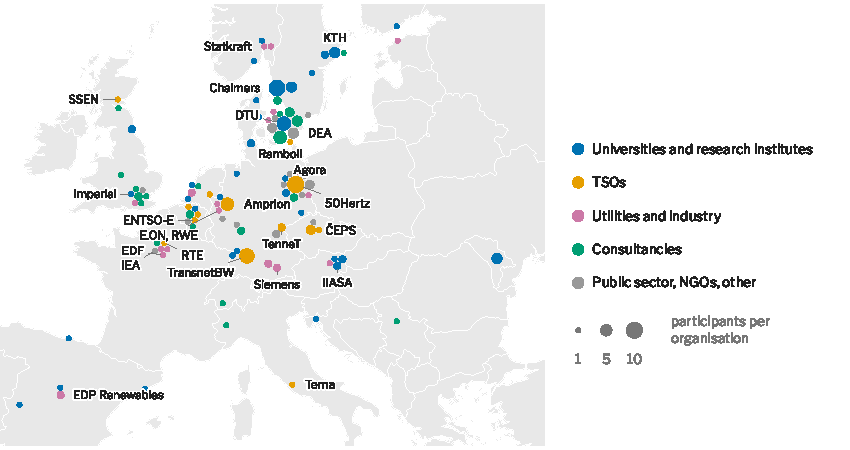
\includegraphics[height=7.5cm]{graphics/final-workshop/participant-map.pdf}
	\begin{tikzpicture}[remember picture, overlay]
		\node[anchor=north west, inner sep=0pt, align=left, text=tub-red, font=\usebeamerfont{frametitle}]
		at ([xshift=10.3cm, yshift=-1.05cm]current page.north west) {Where participants\\came from};
	\end{tikzpicture}
	\source{Anonymised registration list of the 2025 workshops; organisations placed at their head offices.}
\end{frame}

% BEYOND
\section{Beyond}
\begin{frame}{Open tools and models as a basis for public decisions}
	\centering
	\vspace{-0.75em}
	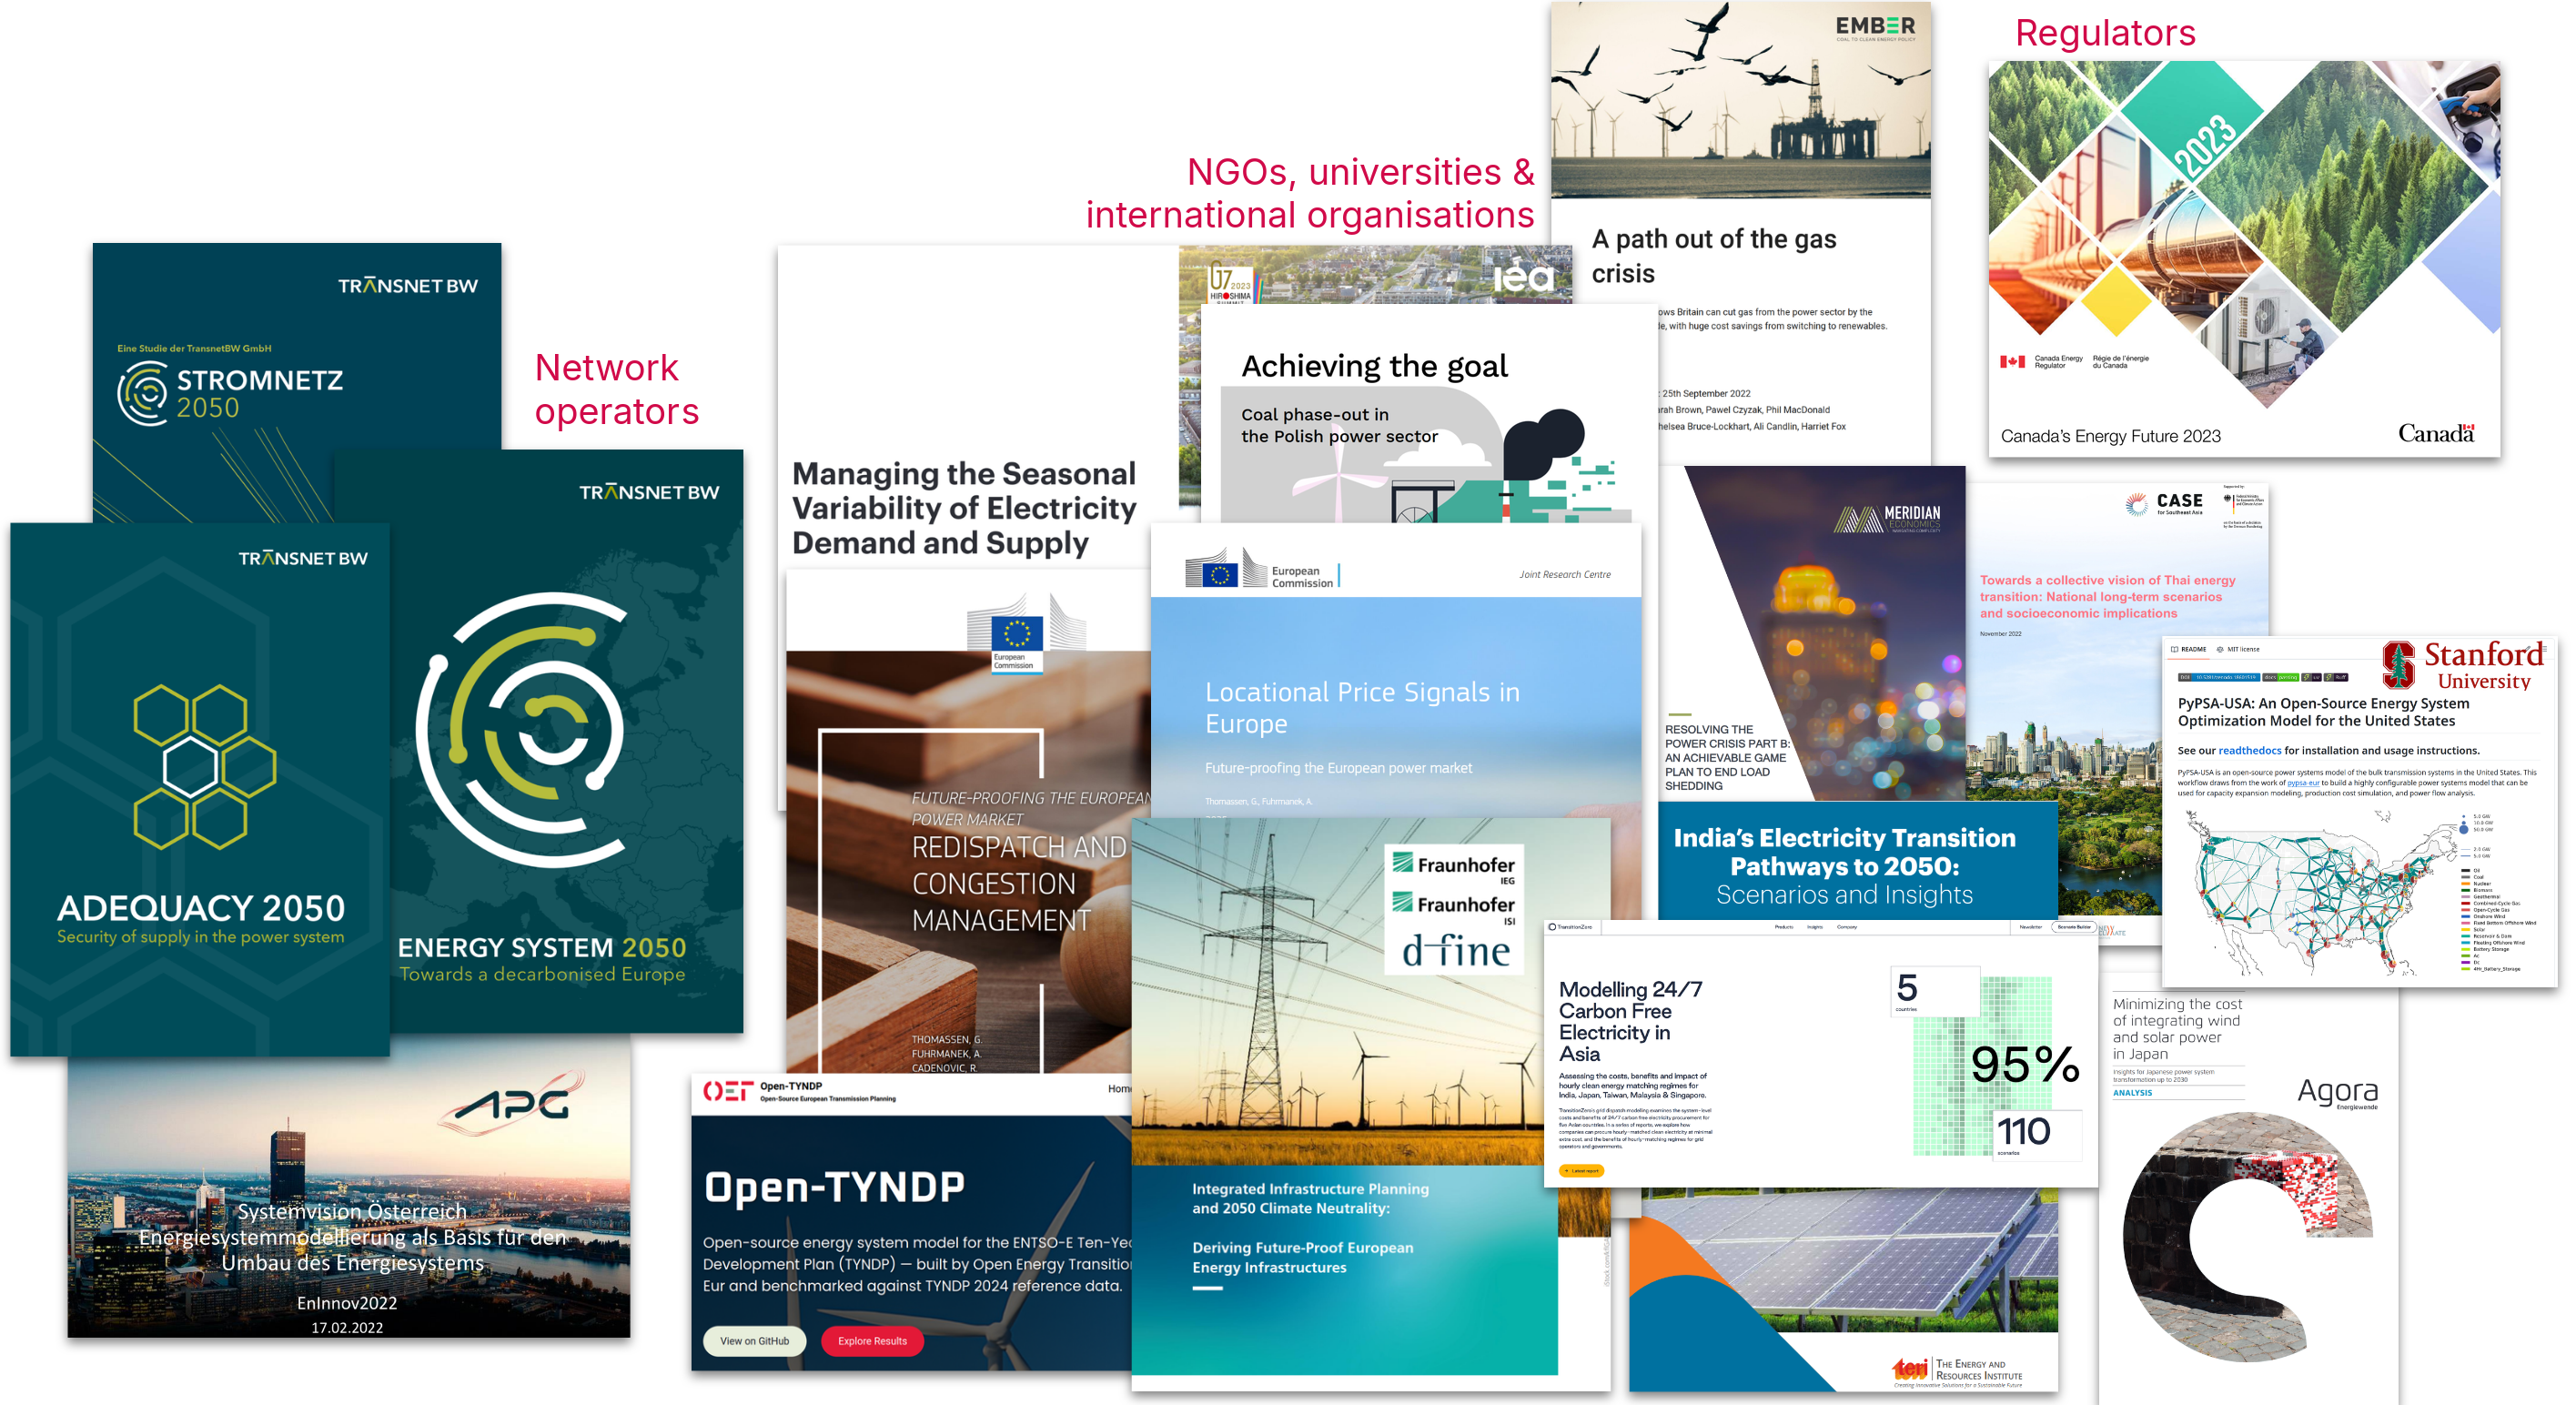
\includegraphics[height=7.0cm]{graphics/final-workshop/who-else-uses-pypsa.png}
\end{frame}

\begin{frame}{RESILIENT in summary}
	\vspace{0.3em}
	\begin{columns}[c,onlytextwidth]
		\begin{column}{0.64\textwidth}
			\placeholder{8.8cm}{5.0cm}{Summary content, to be decided}
		\end{column}
		\begin{column}{0.32\textwidth}
			\centering
			\qrcode[height=3.4cm]{https://resilient-project.github.io/}\\[0.5cm]
			\small\href{https://resilient-project.github.io/}{resilient-project.github.io}
		\end{column}
	\end{columns}
\end{frame}

\end{document}
